


\tikzset{every picture/.style={line width=0.75pt}} %set default line width to 0.75pt        

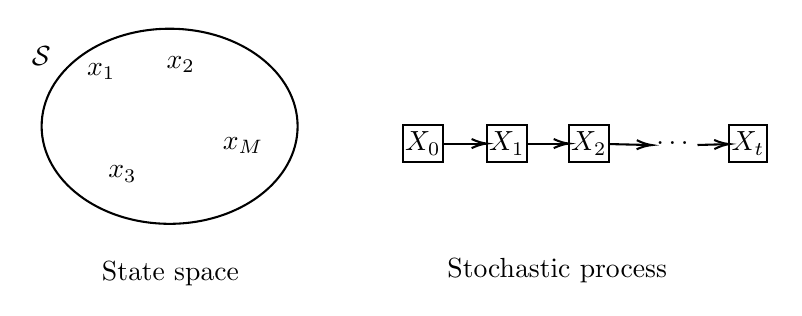
\begin{tikzpicture}[x=0.50pt,y=0.50pt,yscale=-1,xscale=1]
%uncomment if require: \path (0,928); %set diagram left start at 0, and has height of 928

%Shape: Ellipse [id:dp18659796531361872] 
\draw   (59.33,412.31) .. controls (59.33,373.38) and (100.75,341.81) .. (151.83,341.81) .. controls (202.92,341.81) and (244.33,373.38) .. (244.33,412.31) .. controls (244.33,451.25) and (202.92,482.81) .. (151.83,482.81) .. controls (100.75,482.81) and (59.33,451.25) .. (59.33,412.31) -- cycle ;

% Text Node
\draw (50,352.15) node [anchor=north west][inner sep=0.75pt]    {$\mathcal{S}$};
% Text Node
\draw (100.67,507.81) node [anchor=north west][inner sep=0.75pt]   [align=left] {State space};
% Text Node
\draw (90,364.48) node [anchor=north west][inner sep=0.75pt]    {$x_{1}$};
% Text Node
\draw (147.33,359.81) node [anchor=north west][inner sep=0.75pt]    {$x_{2}$};
% Text Node
\draw (105.33,438.81) node [anchor=north west][inner sep=0.75pt]    {$x_{3}$};
% Text Node
\draw (142,404.15) node [anchor=north west][inner sep=0.75pt]    {$\dotsc $};
% Text Node
\draw (188,418.15) node [anchor=north west][inner sep=0.75pt]    {$x_{M}$};
% Text Node
\draw  [line width=0.75]   (320.36,411.31) -- (349.36,411.31) -- (349.36,438.31) -- (320.36,438.31) -- cycle  ;
\draw (334.86,424.81) node    {$X_{0}$};
% Text Node
\draw    (381.03,411.31) -- (410.03,411.31) -- (410.03,438.31) -- (381.03,438.31) -- cycle  ;
\draw (395.53,424.81) node    {$X_{1}$};
% Text Node
\draw    (440.36,411.31) -- (469.36,411.31) -- (469.36,438.31) -- (440.36,438.31) -- cycle  ;
\draw (454.86,424.81) node    {$X_{2}$};
% Text Node
\draw    (556.37,411.31) -- (583.37,411.31) -- (583.37,438.31) -- (556.37,438.31) -- cycle  ;
\draw (569.87,424.81) node    {$X_{t}$};
% Text Node
\draw (501.33,420.81) node [anchor=north west][inner sep=0.75pt]    {$\dots $};
% Text Node
\draw (350.33,505.81) node [anchor=north west][inner sep=0.75pt]   [align=left] {Stochastic process};
% Connection
\draw    (349.36,424.81) -- (379.03,424.81) ;
\draw [shift={(381.03,424.81)}, rotate = 180] [color={rgb, 255:red, 0; green, 0; blue, 0 }  ][line width=0.75]    (10.93,-3.29) .. controls (6.95,-1.4) and (3.31,-0.3) .. (0,0) .. controls (3.31,0.3) and (6.95,1.4) .. (10.93,3.29)   ;
% Connection
\draw    (410.03,424.81) -- (438.36,424.81) ;
\draw [shift={(440.36,424.81)}, rotate = 180] [color={rgb, 255:red, 0; green, 0; blue, 0 }  ][line width=0.75]    (10.93,-3.29) .. controls (6.95,-1.4) and (3.31,-0.3) .. (0,0) .. controls (3.31,0.3) and (6.95,1.4) .. (10.93,3.29)   ;
% Connection
\draw    (469.36,425.16) -- (498.33,425.86) ;
\draw [shift={(500.33,425.91)}, rotate = 181.39] [color={rgb, 255:red, 0; green, 0; blue, 0 }  ][line width=0.75]    (10.93,-3.29) .. controls (6.95,-1.4) and (3.31,-0.3) .. (0,0) .. controls (3.31,0.3) and (6.95,1.4) .. (10.93,3.29)   ;
% Connection
\draw    (533.33,425.85) -- (554.37,425.25) ;
\draw [shift={(556.37,425.19)}, rotate = 538.38] [color={rgb, 255:red, 0; green, 0; blue, 0 }  ][line width=0.75]    (10.93,-3.29) .. controls (6.95,-1.4) and (3.31,-0.3) .. (0,0) .. controls (3.31,0.3) and (6.95,1.4) .. (10.93,3.29)   ;

\end{tikzpicture}